Na równi pochyłej o kącie nachylenia \emph{$\alpha$} znajdują się dwa ciała, z których jedno jest zaopatrzone w~dynamometr. Obliczyć, jaką siłę będzie wskazywał dynamometr, jeżeli ciało o masie \emph{$m_1$} porusza się z tarciem (współczynnik tarcia wynosi $\mu$), a~ciało \emph{$m_2$} porusza się bez tarcia.
\begin{figure}[H]
	\centering
	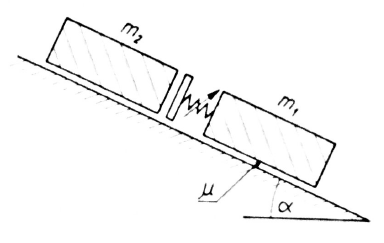
\includegraphics[width=0.3\linewidth]{../rysunki/dynamika/dynamometr-dwa-klocki}
\end{figure}

%Kruczek 5_16R/50
%Poziom B